\chapter{Research Phase}
\section{current modeling environments}

\subsection{simile (Simile Visual Modelling Environment)}
Simile is a visual modelling environment, developed originally for the dynamic modelling of ecological and environmental systems, which supports a wide range of ways of representing space. Therefore, it addresses both of the above issues in a single environment.\footnote{http://www.simulistics.com/index.htm and Book: Re-presenting GIS from Peter Fisher}

\emph{Visual modeling environment}
\begin{itemize}
	\item Build model without learning programming
	\item Display concept \& relationship using diagram, for example (stocks, flows and influences)
	\item GUI for simulation control \& specifying inputs
	\item Visualize \& compare the model behaviors in  graphs \& tables
\end{itemize}

\emph{What can we use it for?}
\begin{itemize}
	\item Rate expressions for biological, chemical, or physical processes (differential equations), for example: Mass balance or accounting, Growth dynamics, Respiration
	\item Scenario analysis, for example: Effect of flow velocity on gas exchange between  river-atmosphere
\end{itemize}

\emph{Simile has a number of features:}
	\subsubsection{Visual modelling:}
Simile supports a two-phase approach to model construction. The first involves the drawing of diagrams that show the main features of the model and the second involves fleshing-out the model-diagram elements with quantitative information on the relevant values and equations.
	\subsubsection{System Dynamics:}
Simile allows models to be formulated in System Dynamics terms, as compartments (stocks, levels) whose values are governed by flows in and out. This can be considered as a visual language for representing differential-equation models, with a compartment representing a state variable, and the rate-of-change being the net sum of inflows minus outflows.
	\subsubsection{Disaggregation:}
Simile allows the modeller to express many forms of disaggregation: e.g. age/size/sex/species classes. This is achieved by defining how one class behaves, then specifying that there are many such classes.
	\subsubsection{Object-based modelling:}
Simile allows a population of objects to be modelled. As with disaggregation, model designers state how one member behaves, then specify that there are many such members. In this case, the designer can add in symbols denoting the rules for creating new members of the population, and for killing off existing members. Individual members of the population can interact with others.
	\subsubsection{Spatial modelling:}
It follows that spatial modelling in the system is simply a special form of disaggregation. One spatial unit (grid square, hexagon, polygon, etc.) is modelled, then many such units are specified. Each can be given spatial attributes, such as area or location, and the proximity of one unit to another can be represented.
	\subsubsection{Modular modelling:}
Simile allows any model to be inserted as a submodel into another. Having done this, the modeller can then manually make the links between variables in the two components (in the case where the submodel was not designed to plug into the main model); or links can be made automatically, giving a (plug-and-play) capability. Conversely, any submodel can be extracted and run as a stand-alone model, greatly facilitating testing of the submodels of a complex model.
	\subsubsection{Efficient computation:}
Models can be run as compiled programs. In many cases, these will run as fast as a hand-coded program, enabling Simile to cope with complex models (100s equations; 1000s object instances). While larger or institutional spatial databases are likely to contain millions of object instances, the complexity of modelling, rather than the efficiency of computation, means that dynamic spatial modelling tasks are often more modest in size.
	\subsubsection{Customisable output displays and input tools:}
Simile users can design and implement their own input/output procedures independently. In particular, they can develop displays for model output that are specific to disciplinary norms or other requirements. Once developed, these can be shared with others in the relevant research community.
	\subsubsection{Declarative representation of model structure:}
A Simile model is saved in an open format as a text file (in Prolog syntax). This means that others can develop tools for processing Simile models in novel ways. For example, one group may develop a new way of reporting on model structure, while another may wish to undertake automatic comparison of the structure of two similar models. It also opens the way for the efficient transmission of models across the Internet (as XML files), and for the sharing of models between different modelling environments.\\
	
In fact, Simile has no particular spatial representations built into it, rather these are specified by the user in Simile's modelling language and this means that modellers have considerable flexibility in just how space is represented. They are not restricted to some pre-defined spatial framework. One model can include both field and object views, polygonal, rectangular and hexagonal areal units, 3D units (e.g. cubes), and point and linear features, all referenced to a common co-ordinate system. Together with appropriate visualisation tools, this flexibility enables a very wide range of dynamic spatial models to be developed.\\
	
\emph{The Simile visual modelling environment allow to:}
\begin{itemize}
	\item draw the elements of model, and the relationships between them
	\item add influences between related variables
	\item using simple mouse actions, to re-arrange the elements, annotate the diagram or add graphics
\end{itemize}	
	
\emph{System Dynamics symbols}
\begin{itemize}
	\item \emph{compartment:}\\
The compartment symbol is used to represent a quantitative state variable
	\item \emph{Flow arrow:}\\
The flow arrow is used to specify a term contributing to the rate of change of a compartment
	\item \emph{Variable:}\\
A variable is used to hold one or more values. The value or values come from a mathematical expression
	\item \emph{Influence arrow :}\\
To say that (A influences B) means that A is used to calculate a value for B
\end{itemize}	

\begin{figure}[htbp]
\centering
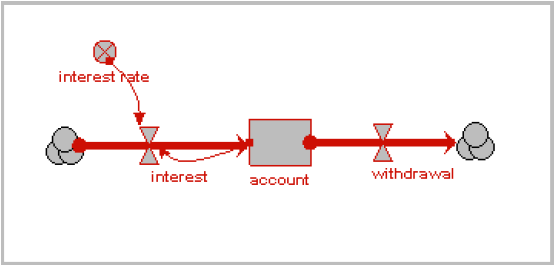
\includegraphics[width=0.5\textwidth]{pics/account_example.png}
\caption{the model diagram}
\label{fig:the model diagram}	
\end{figure}

In common with other visual modelling environments, Simile models are built in two phases. First, the modeller produces a diagram. Then, the modeller quantifies the model by entering numeric values and equations for the various components of the model.\\
The diagramming icons are chosen from the Toolbar of simile, the compartment, flow, variable and influence, are concerned with conventional System Dynamics modelling.\\
System Dynamics (SD) is a common dynamic modelling paradigm within the ecological and environmental research communities. A SD model consists of compartments (stocks, levels, storages) connected by flows, with subsidiary variables for representing parameters and intermediate variables, and influence arrows to show which compartments and variables are used in the calculation of flows and other variables. Essentially, SD is a cosmetic language for defining differential- or difference-equation models: differential equations if the equations are taken to define continuous change; difference equations if the time step is taken to be unity.

\emph{Concern following problems of simile:}
\begin{itemize}
	\item effort and skill needed to program the models
	\item the lack of transparency in models implemented as programs
	\item and the lack of reuseability of models and submodels.
\end{itemize}	
	
\subsection{esmf (Earth System Modeling Framework)}
\emph{What ESMF is being developed?}\\
The ESMF is an abbreviation for Earth System Modeling Framework. ESMF is a registered Open Source project for building climate, numerical weather prediction, data assimilation, and other Earth science software applications. These applications are computationally intensive and usually run on supercomputers. The ESMF project is distinguished by community governance and distributed development, and by a diverse customer base that includes modeling groups from universities, major U.S. research centers, the National Weather Service, the Department of Defense, and NASA [01].\\
ESMF is a component-based software that increases the interoperability of Earth science modeling software developed at different sites and promotes code reuse. The idea of the project is to transform distributed, specialized knowledge and resources into a collaborative, integrated modeling community that operates more efficiently, and is more responsive to societal needs.\footnote{http://en.wikipedia.org/wiki/ESMF and http://www.earthsystemmodeling.org/}

\emph{Architecture}\\
The components within an ESMF software application usually represent large-scale physical domains such as the atmosphere, ocean, cryosphere, or land surface. The components can create and drive other components.\\
The software that connects physical domains is called a coupler in the Earth system modeling community. Couplers are used for taking the outputs from one component and transforming them into the inputs that are needed to run another component. In ESMF, couplers are also software components.

\emph{Capabilities}\\
In ESMF, user data are represented in the form of data objects such as grids, fields, and arrays. The user data within a component may be copied or referenced into these ESMF objects.\\
ESMF can associate metadata with data objects. The metadata, in the form of name and value pairs, is grouped into packages. These metadata packages can be written out in XML and other standard formats.

\emph{Features}\\
The ESMF differs from other published existing frameworks in the following features:
\begin{itemize}
	\item Full Fortran 90 interface, partial C/C++ interface
	\item Fortran 90 Reference Manual and User's Guide
	\item Runs on most high performance parallel computing platforms, including IBM, many Linux variants, Cray, Compaq, more
	\item Supports MPI, OpenMP and hybrid user codes
	\item Free user support
	\item Active user community[02]
\end{itemize}

\emph{Disadvantages}\\
The ESMF includes user manuals, which should help the beginners to gain entry into the application of the framework. The disadvantage of the manuals is that they are too large and too complex. This complicates the use of the framework.
Although there is FAQ on the website of ESMF, which answers the most frequently asked questions, but there is not a forum where people can share their questions and answers.

\subsection{oms (Object Modeling System)}
\emph{What is OMS?}\\
OMS stands for object oriented framework for environmental modeling implemented by java. With OMS, scientists can build scientific model, components efficiently.\\
It is a collaborative project carried out by US Department of Agriculture and other partner organizations, which are involved in agro-environmental modeling. The goal of OMS is to provide features to the modelers to create inter-operable, scalable models that take full advantage of contemporary computing, management and infrastructure technologies while keeping it simple and intuitive for users.

\emph{What is OMS good for?}\\
OMS supports component based software engineering. Models and components are regarded as objects in OMS. The OMS framework introduces a new style of component modelling. No interface should be implemented. OMS uses Meta data with annotations to specify the input and output. This new kind of annotations makes it easier for modelers to identify the interactions of different components. The modelers will have a better overview of each component. Data flow through the components will be clearer for them. The modelers can profit from this feature to create a large component combining different subcomponents to fulfill a complicated task.\\
The OMS framework provides simulations features for modelers to test the model created by them. Simulations are model applications. It consists of model, input data, output management, execution type, execution environment. OMS provides a DSL to run the simulations. DSL is a mini-language that represents constructs of a given domain. With a DSL, simulations can be created from different tools, for example, IDEs, OMS console. With the simulation feature, the modelers are able to evaluate and improve their models.
OMS provides diagram visualization of the simulation results. Modelers can use this feature to get a deeper insight of the functions of their models.\\
OMS is designed to support delivery of science relating to agricultural and natural resource management. It is so versatile usable that it can inter-operate with other frameworks of agricultural modeling worldwide.

\emph{What is the disadvantages of OMS?}\\
\begin{itemize}
	\item Not stable. Many exceptions
	\item Little help documentations
	\item Costs much time to make OMS work
\end{itemize}

\section{problems}
\section{declarative modelling}
\section{semantic approaches}